\chapter{\texttt{RAFFT} Appendices}

\section{\texttt{RAFFT} example calls}

\texttt{RAFFT}  computes the fast-folding paths for a given sequence. Starting from the wholly unfolded structure, it quickly identifies stems using the FFT-based technique.

For example, we can use the following commands on the Coronavirus frameshifting stimulation element obtained from RFAM:

\noindent to display only the final structures

\noindent \rule{12cm}{0.4pt}
\begin{lstlisting}[language=bash, caption={Command line to run \texttt{RAFFT} executable after installation}]
$ rafft -s GGGUUUGCGGUGUAAGUGCAGCCCGUCUUACACCGUGCGGCACAGGCA 
-ms 5 
\end{lstlisting}
\rule{12cm}{0.4pt}

\noindent to display the visited/saved intermediates

\noindent \rule{12cm}{0.4pt}
\begin{lstlisting}[language=bash, caption={Command line to run \texttt{RAFFT} executable after installation}]
$ rafft -s GGGUUUGCGGUGUAAGUGCAGCCCGUCUUACACCGUGCGGCACAGGCA 
-ms 5 
--traj
\end{lstlisting}
\rule{12cm}{0.4pt}

\noindent The result to this call could look like this: 

\noindent \rule{12cm}{0.4pt}
\begin{lstlisting}[language=bash, caption={\texttt{RAFFT}'s output results}]
GGGUUUGCGGUGUAAGUGCAGCCCGUCUUACACCGUGCGGCACAGGCA
# ---------0----------
................................................    0.0
# ---------1----------
.....(((((((((((..........)))))))))))...........  -14.0
(((((..............)))))........................   -4.6
...............((((....................)))).....   -3.4
....(((((.......)))))...........................   -2.8
......((((............))))......................   -2.5
# ---------2----------
..((((((((((((((.((.....))))))))))))).))).......  -15.8
.....(((((((((((.((.....)))))))))))))..((....)).  -15.5
.....(((((((((((..........)))))))))))...........  -14.0
(((((.(((.......))))))))...........(((.......)))  -11.2
(((((.(((.......))))))))((((...............)))).  -10.4
# ---------3----------
..((((((((((((((.((.....))))))))))))).))).......  -15.8
.....(((((((((((.((.....)))))))))))))..((....)).  -15.5
.....(((((((((((..........)))))))))))...........  -14.0
(((((.(((.......))))))))((((....((....))...)))).  -13.0
(((((.(((.......))))))))((((......(((...))))))).  -11.2
\end{lstlisting}
\noindent \rule{12cm}{0.4pt}

\noindent where the columns shows respectively the predicted structures and their free energies.

\section{Kinetic comparison}
\label{app:sec:kinetic}
According to the RNA structure thermodynamics, one RNA molecule can adopt a
structure $\mathcal{S}$ with probability $p(\mathcal{S}) \propto \text{exp}(-\beta \Delta G(\mathcal{S}))$,
where \(\beta\) is the inverse thermal energy (mol/kcal). To measure the quality
of the ensemble of structures proposed by our method, we measured: (1) the
average probability of each structures in the ensemble, then (2) the diversity
of these structures.

The probability coverage $PC$ given by $PC(\mathcal{S}) = \frac{1}{|\Omega|}\sum_{\mathcal{S}\in
	\Sigma} p(\mathcal{S})$. $\Omega$ is the ensemble of structures sampled by a given
method. We compared, for various random sequences, the probability coverage to
methods based on Boltzmann sampling
\cite{hofacker03_vienn_rna_secon_struc_server,entzian2021rnaxplorer}. We
generated ensembles of $10^2, 10^3$, and $10^4$ structures per sequence denoted
respectively SB100, SB1K, and SB10K. In addition, we also compared to
\texttt{RNAxplorer}, a tool also based on a biased Boltzmann sampling.

\begin{figure}[t!] \centering
	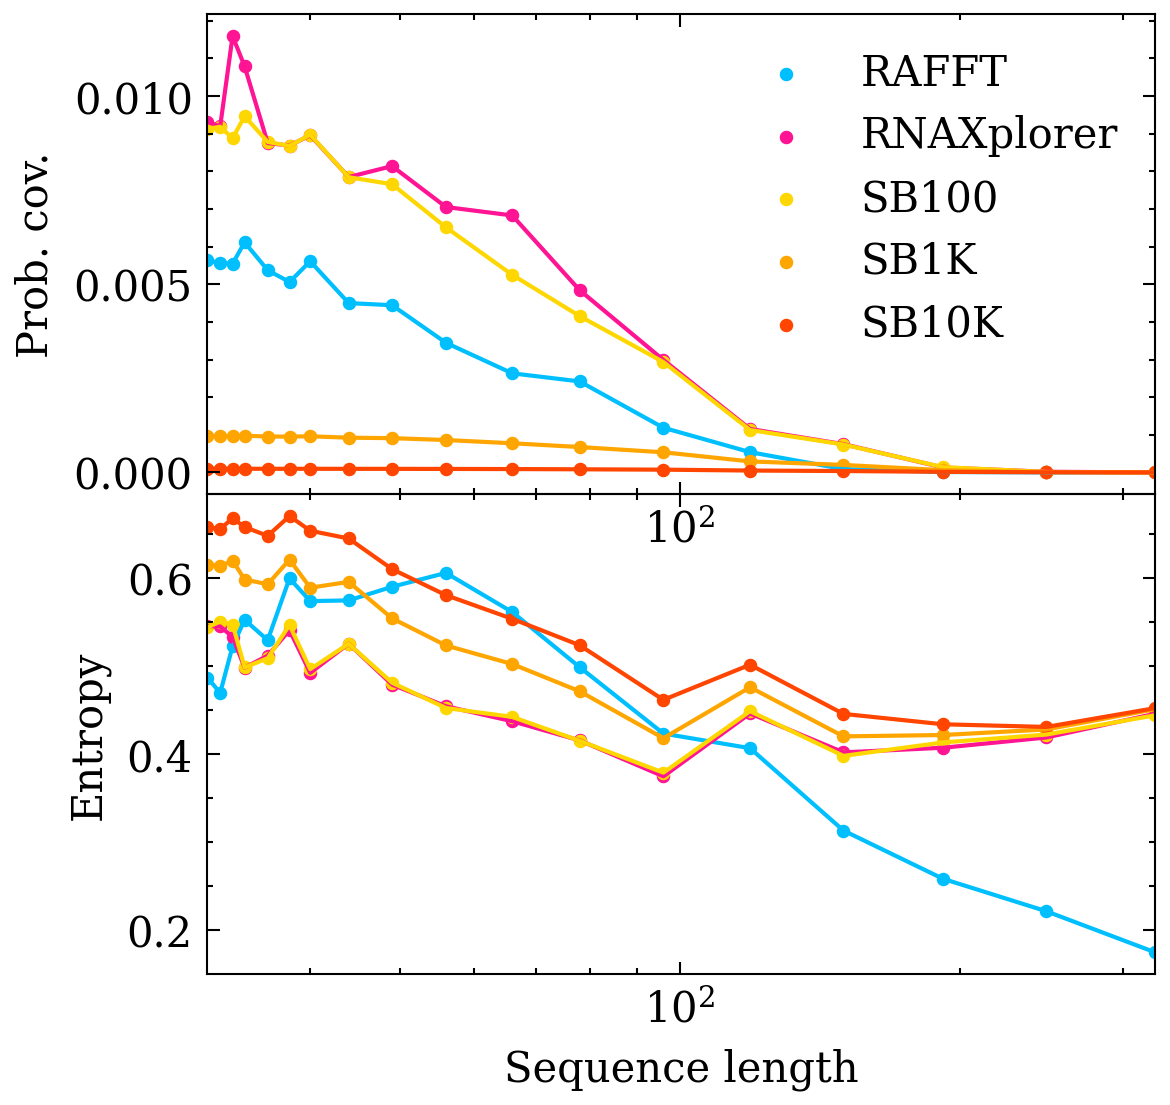
\includegraphics[width=1.\linewidth]{../res/images/rafft/prob_ent.png}
	\caption{\label{struct_ens_char}\textbf{Structure ensemble characterization.} The upper
		part shows the average probability summed over the ensembles of structures
		predicted per sequence with different methods. The bottom part shows the
		average positional entropy of structures using the dot-bracket notation.}
\end{figure}

All structures are represented in the dot-bracket notation. In the dot-bracket
notation, one structure has $\Delta_{\sigma}=\{(, ., )\}$ symbols at each position. Given
these three symbols, we propose the following positional entropy measure
$\Delta S=\frac{1}{L}\sum f_i(\Delta_{\sigma}) \times \text{log}(f_i(\Delta_{\sigma}))$, where $f_i(\Delta_{\sigma})$ is the frequency of a symbol $\delta_{\sigma}$ at position $i$ in the ensemble of structure proposed.

Figure \ref{struct_ens_char} shows the probability coverage and the positional
entropy measure per method. It shows comparable sampling performances for fairly
size sequences ($\approx 10^2$ nucleotides); and a comparable diversity.

\section{\texttt{RAFFT} performance analysis for a stacking size of $200$}
The heuristic method implemented in \texttt{RAFFT} relies on two critical parameters: the stacking size and the number of positional lag. In this section, we analyse the performance of \texttt{RAFFT} for 100 positional lags and 200 secondary structures stored in the stack. \autoref{app:perf_fig} shows the performance of \texttt{RAFFT} compared to both \ac{ML} (\texttt{Mxfold2}) and \ac{MFE} (\texttt{RNAfold}) methods. When choosing the best of the 200 predictions, \texttt{RAFF} performance is similar to \texttt{RNAfold} whereas, \texttt{Mxfold} outperformed both \texttt{RAFFT} and \texttt{RNAfold}. 
\hspace{-2cm}
\begin{figure}[t!]
	\centering
	\subfloat[]{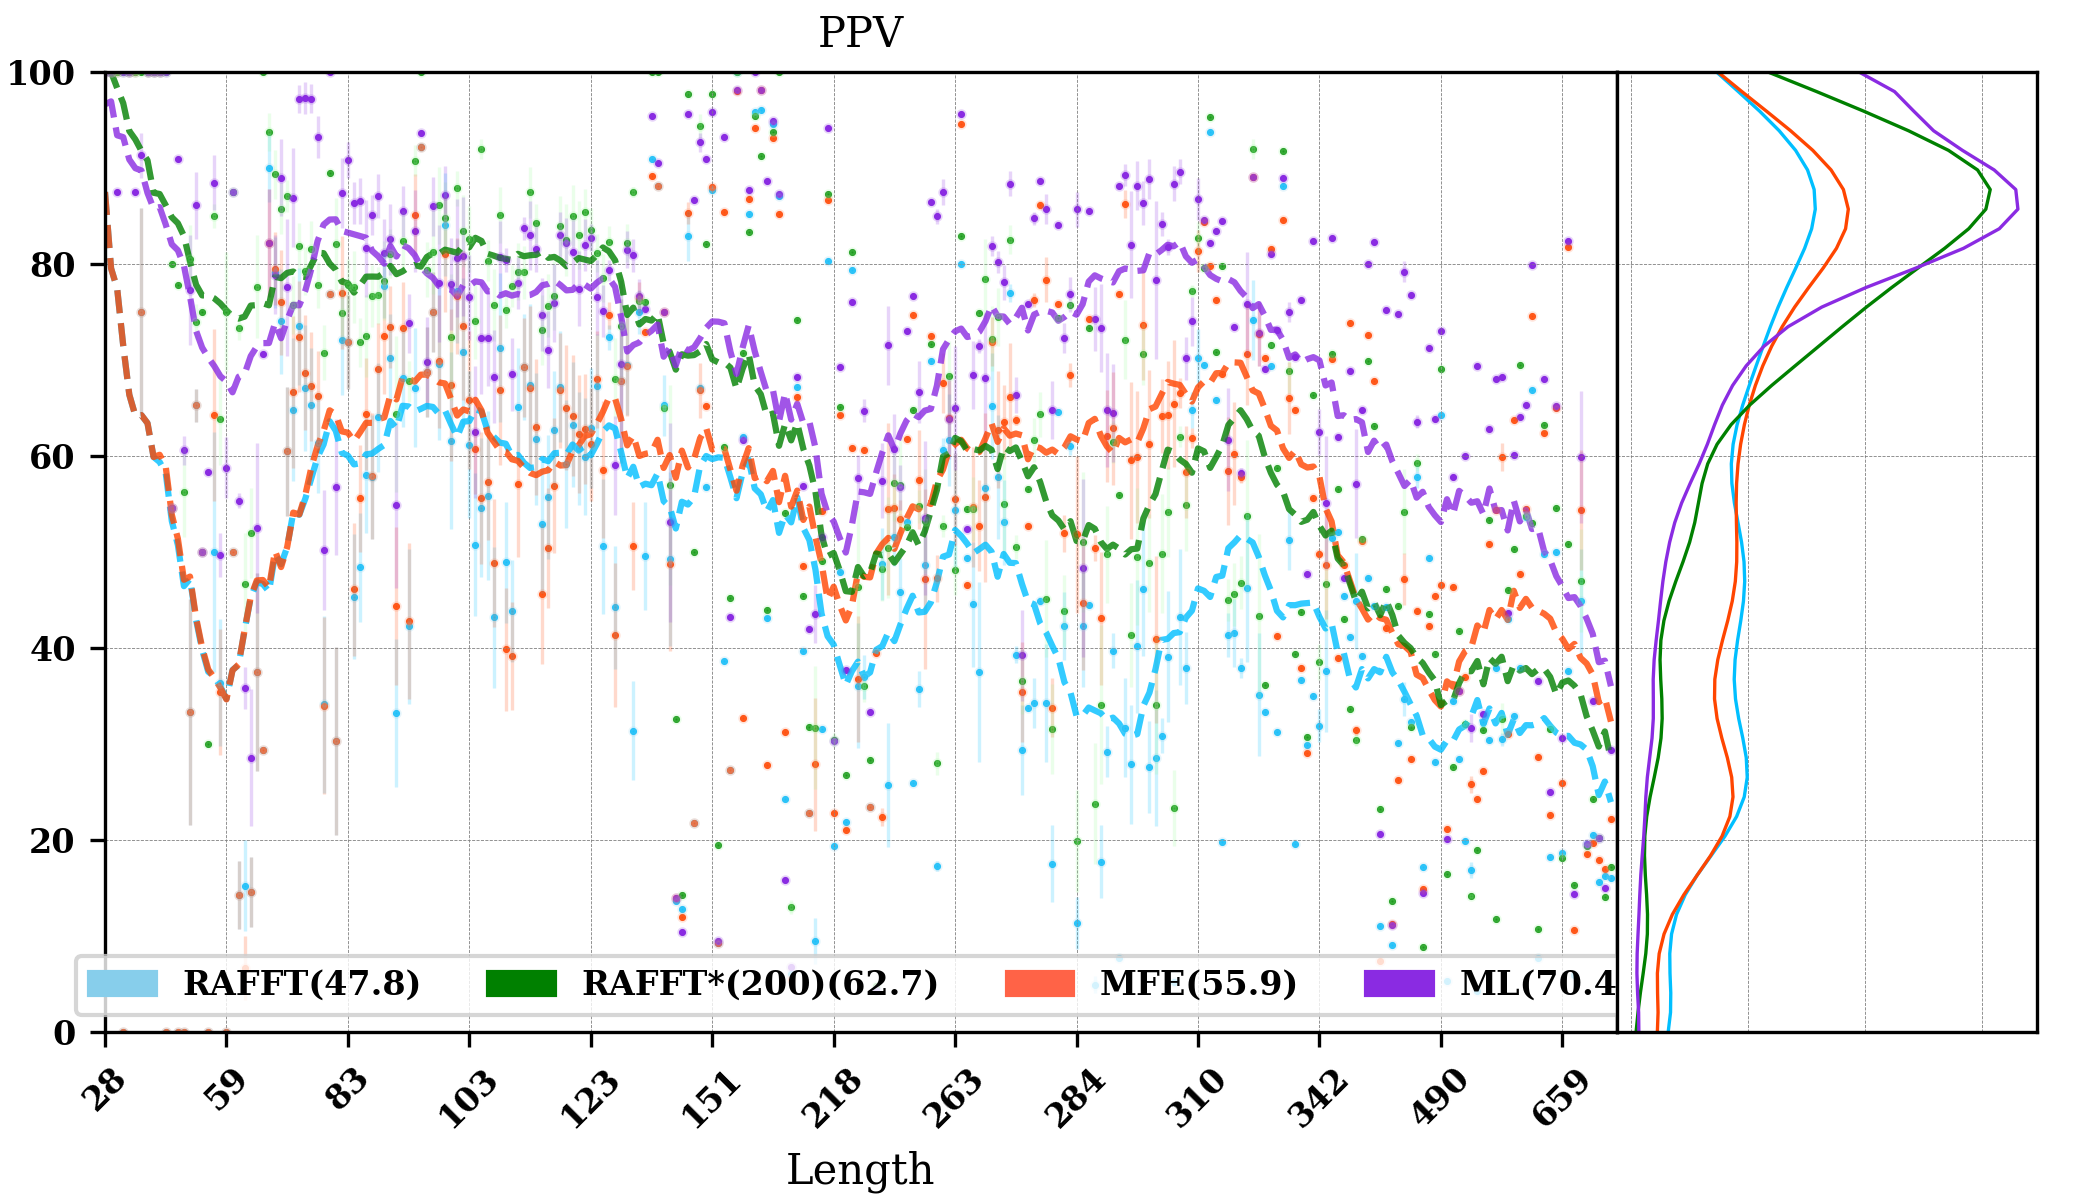
\includegraphics[scale=.7]{../res/images/rafft/fold_perf_ppv_200.png}}\\
	%\hspace{-2cm}
	\subfloat[]{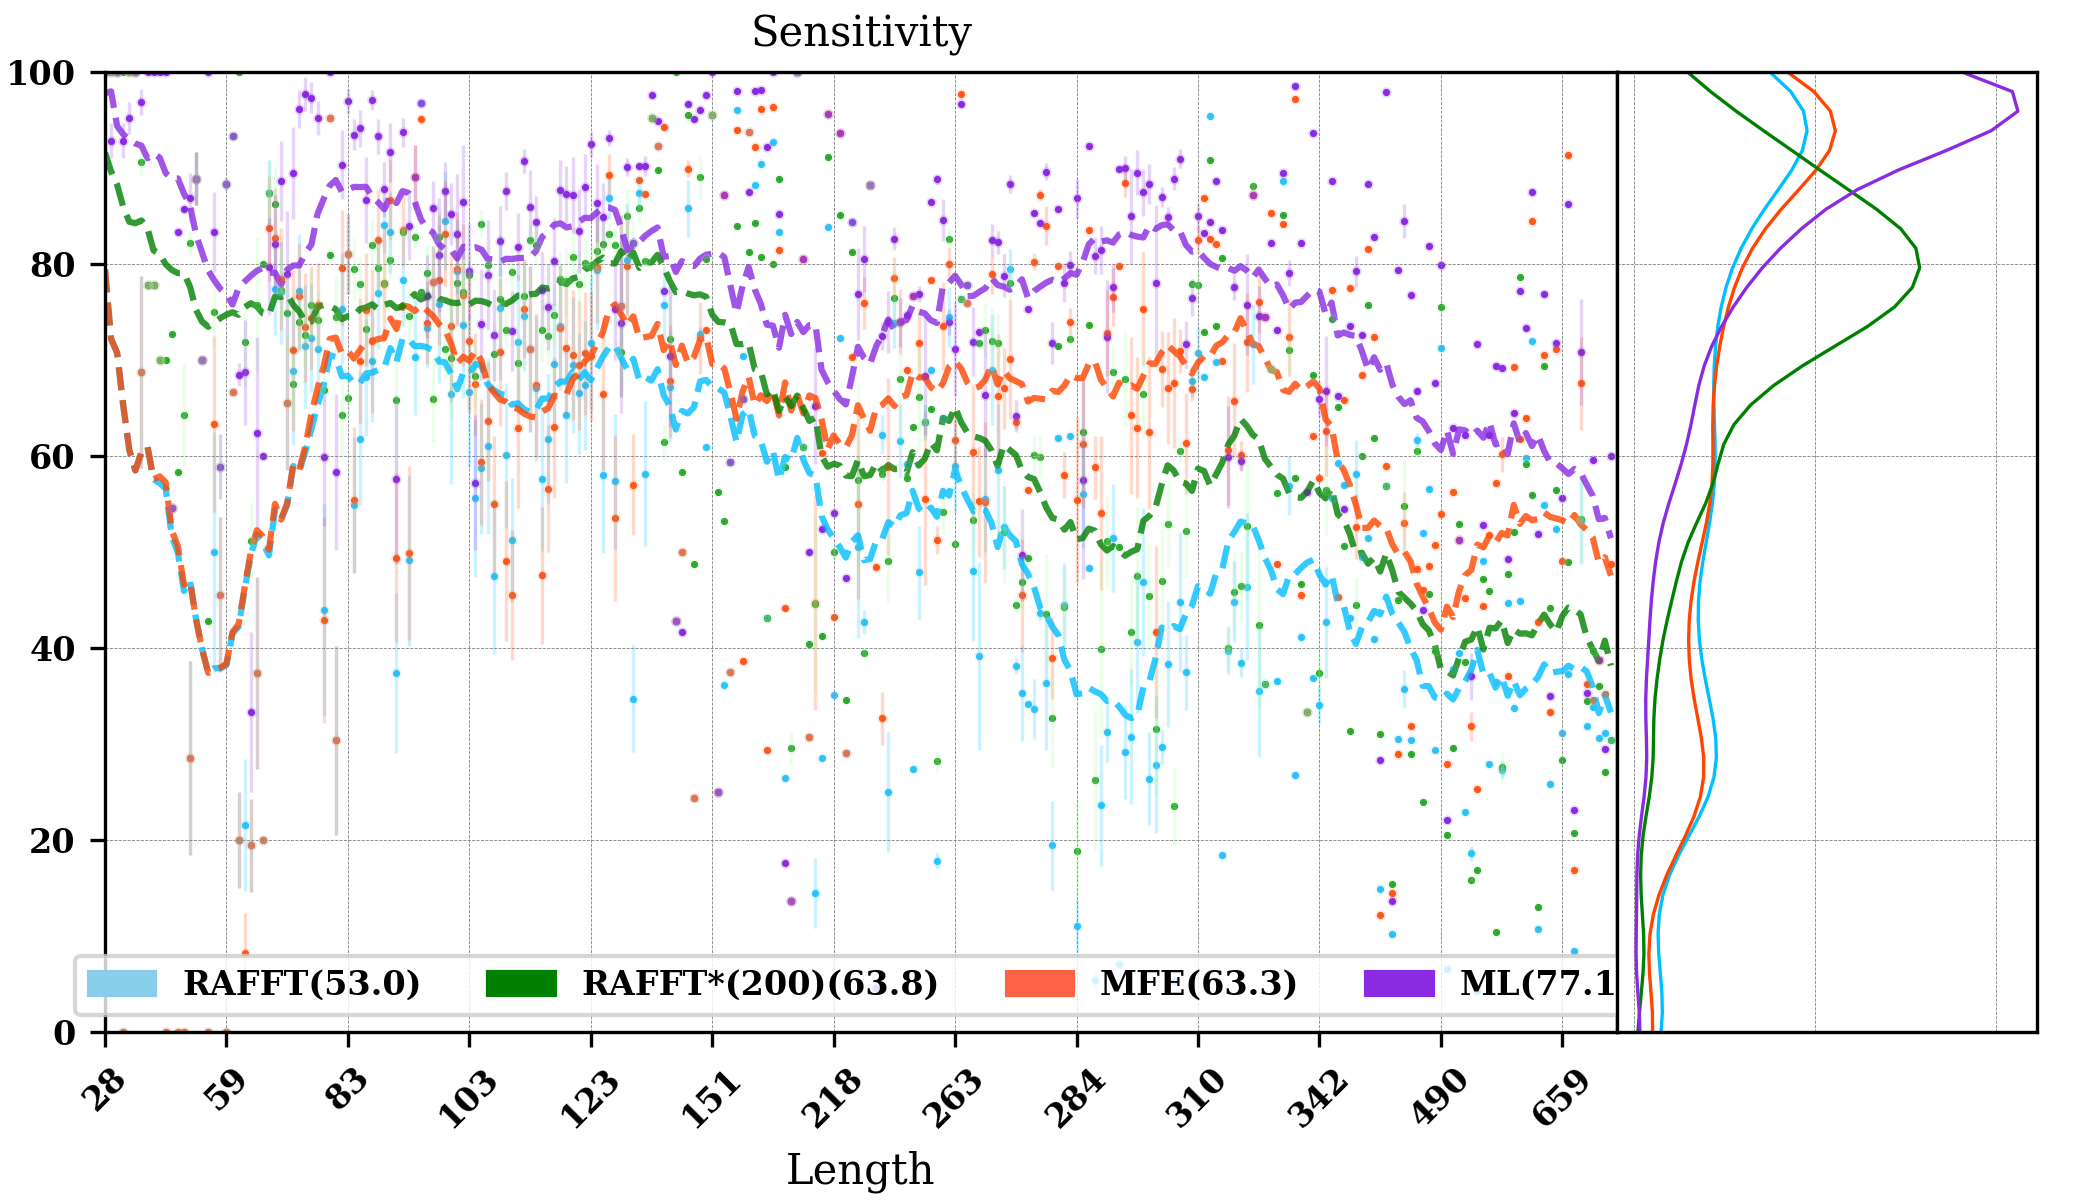
\includegraphics[scale=.7]{../res/images/rafft/fold_perf_sens_200.png}}
	\caption{\textbf{Positive predictive values and sensitivity results\label{app:perf_fig}.}
		RAFFT (blue) displayed the best energy found. RAFFT*(200) shows the best score found among 200 saved structures. Left pans show the density (sequence-wise) of the accuracy measures.}
\end{figure}

\section{\texttt{RAFFT} performance analysis with various values of loop minimum energy contribution}
Structures are added to the stacks by searching for a consecutive number of base-pairs for each selected positional lag. In the best case, it forms a stem, but in some cases, when the base-pairs are not consecutive, different loops are formed, i.e. bulges or hairpins. Therefore, adding a loop to the existing structure depends on its energy contribution. For a loop to be added to the current secondary structure, its energy should be less than a threshold value. In this section, we analyse the influence of this parameter on \texttt{RAFFT} performance. \autoref{app:perf_min_energy} show the \ac{PPV} and sensitivity performances with respect to the sequence lengths. The results show similar performance for loop energy parameters taken from $0$ to $5$.
\begin{figure}[t!]
	%\hspace{-4cm}
	\subfloat[]{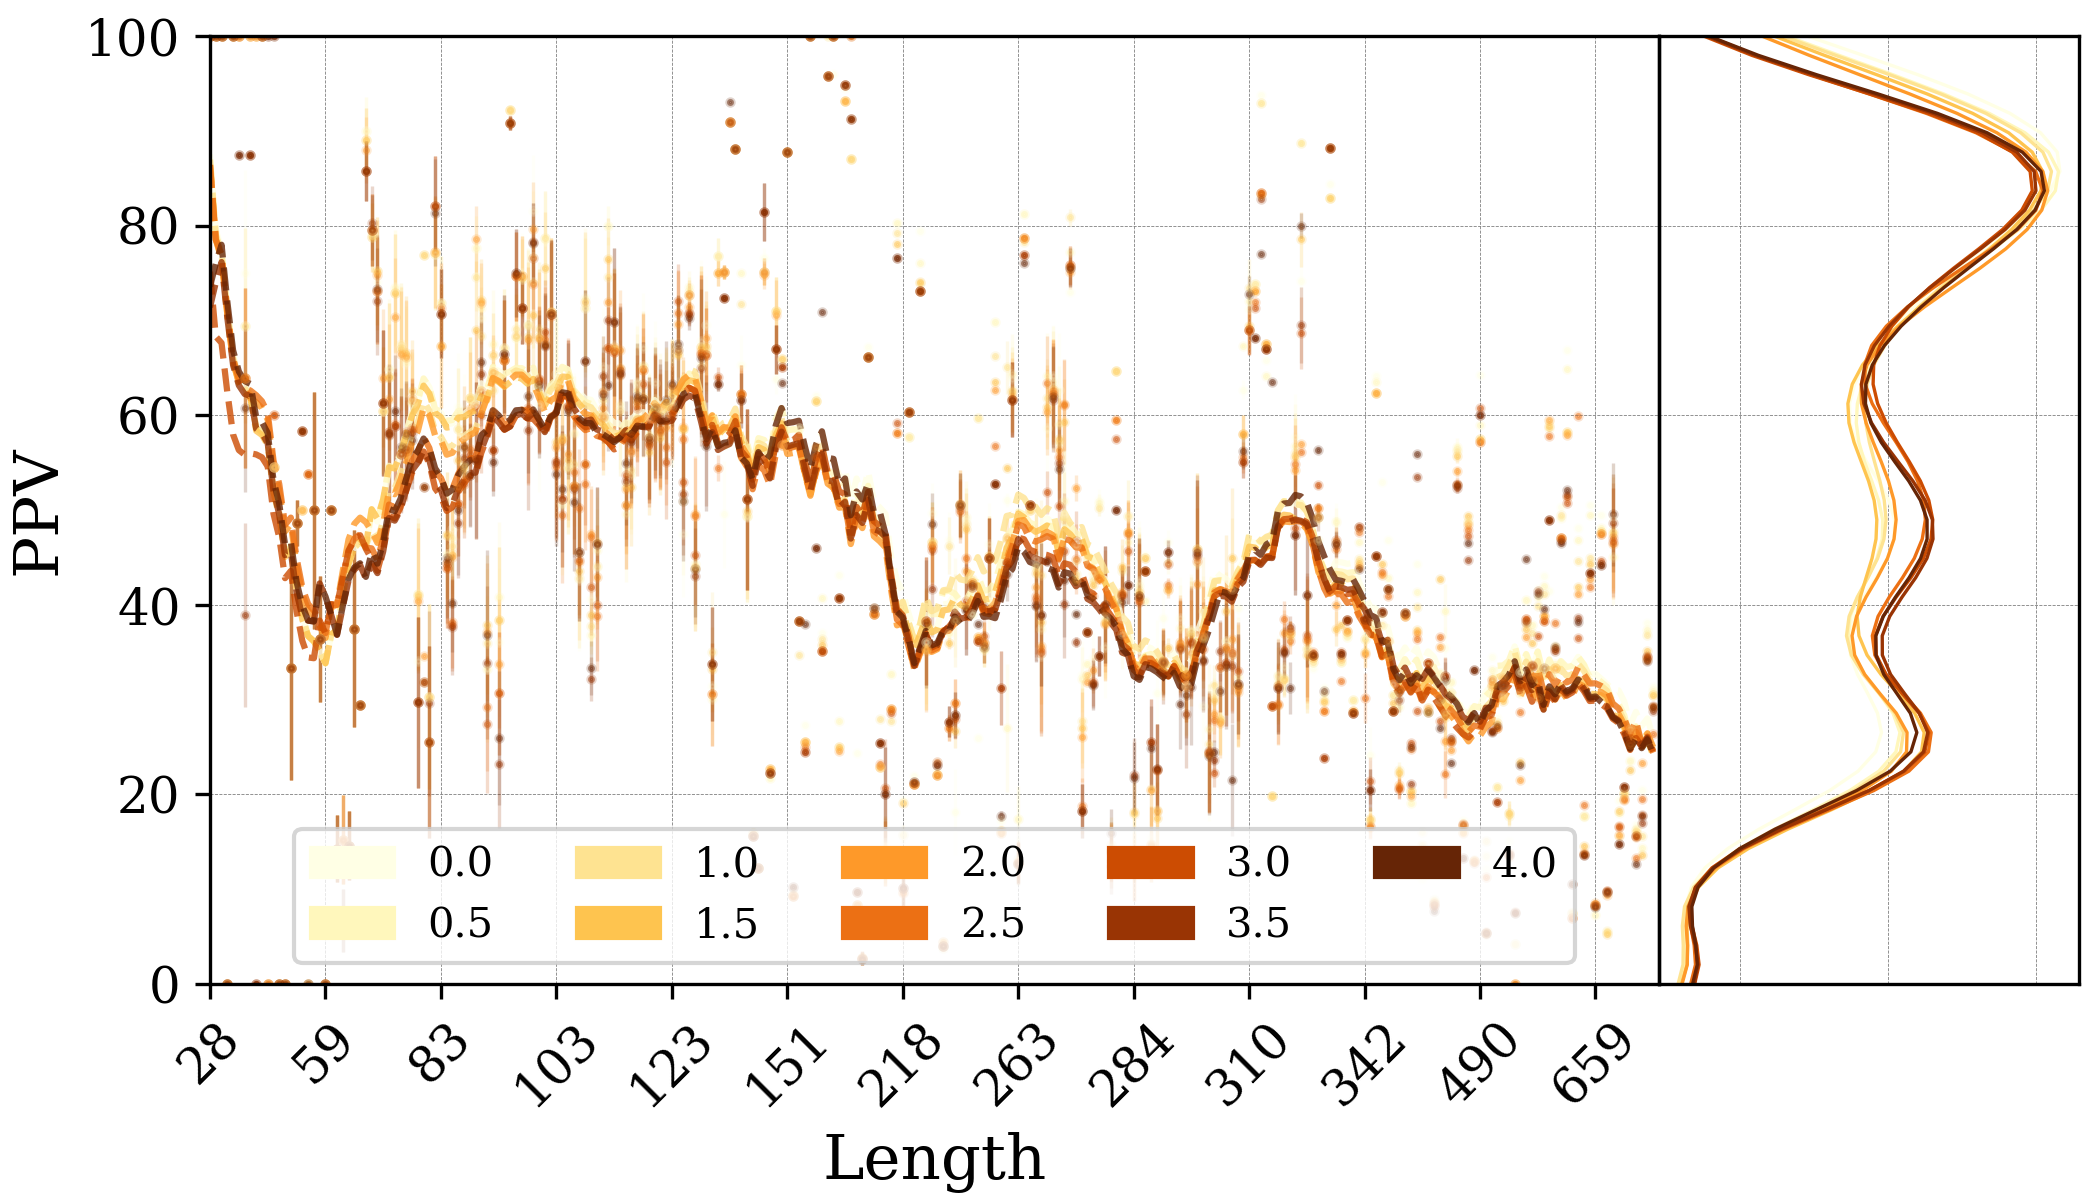
\includegraphics[scale=.7]{../res/images/rafft/rafft_perf_ppv_minenergy.png}}\\
	%\hspace{-4cm}
	\subfloat[]{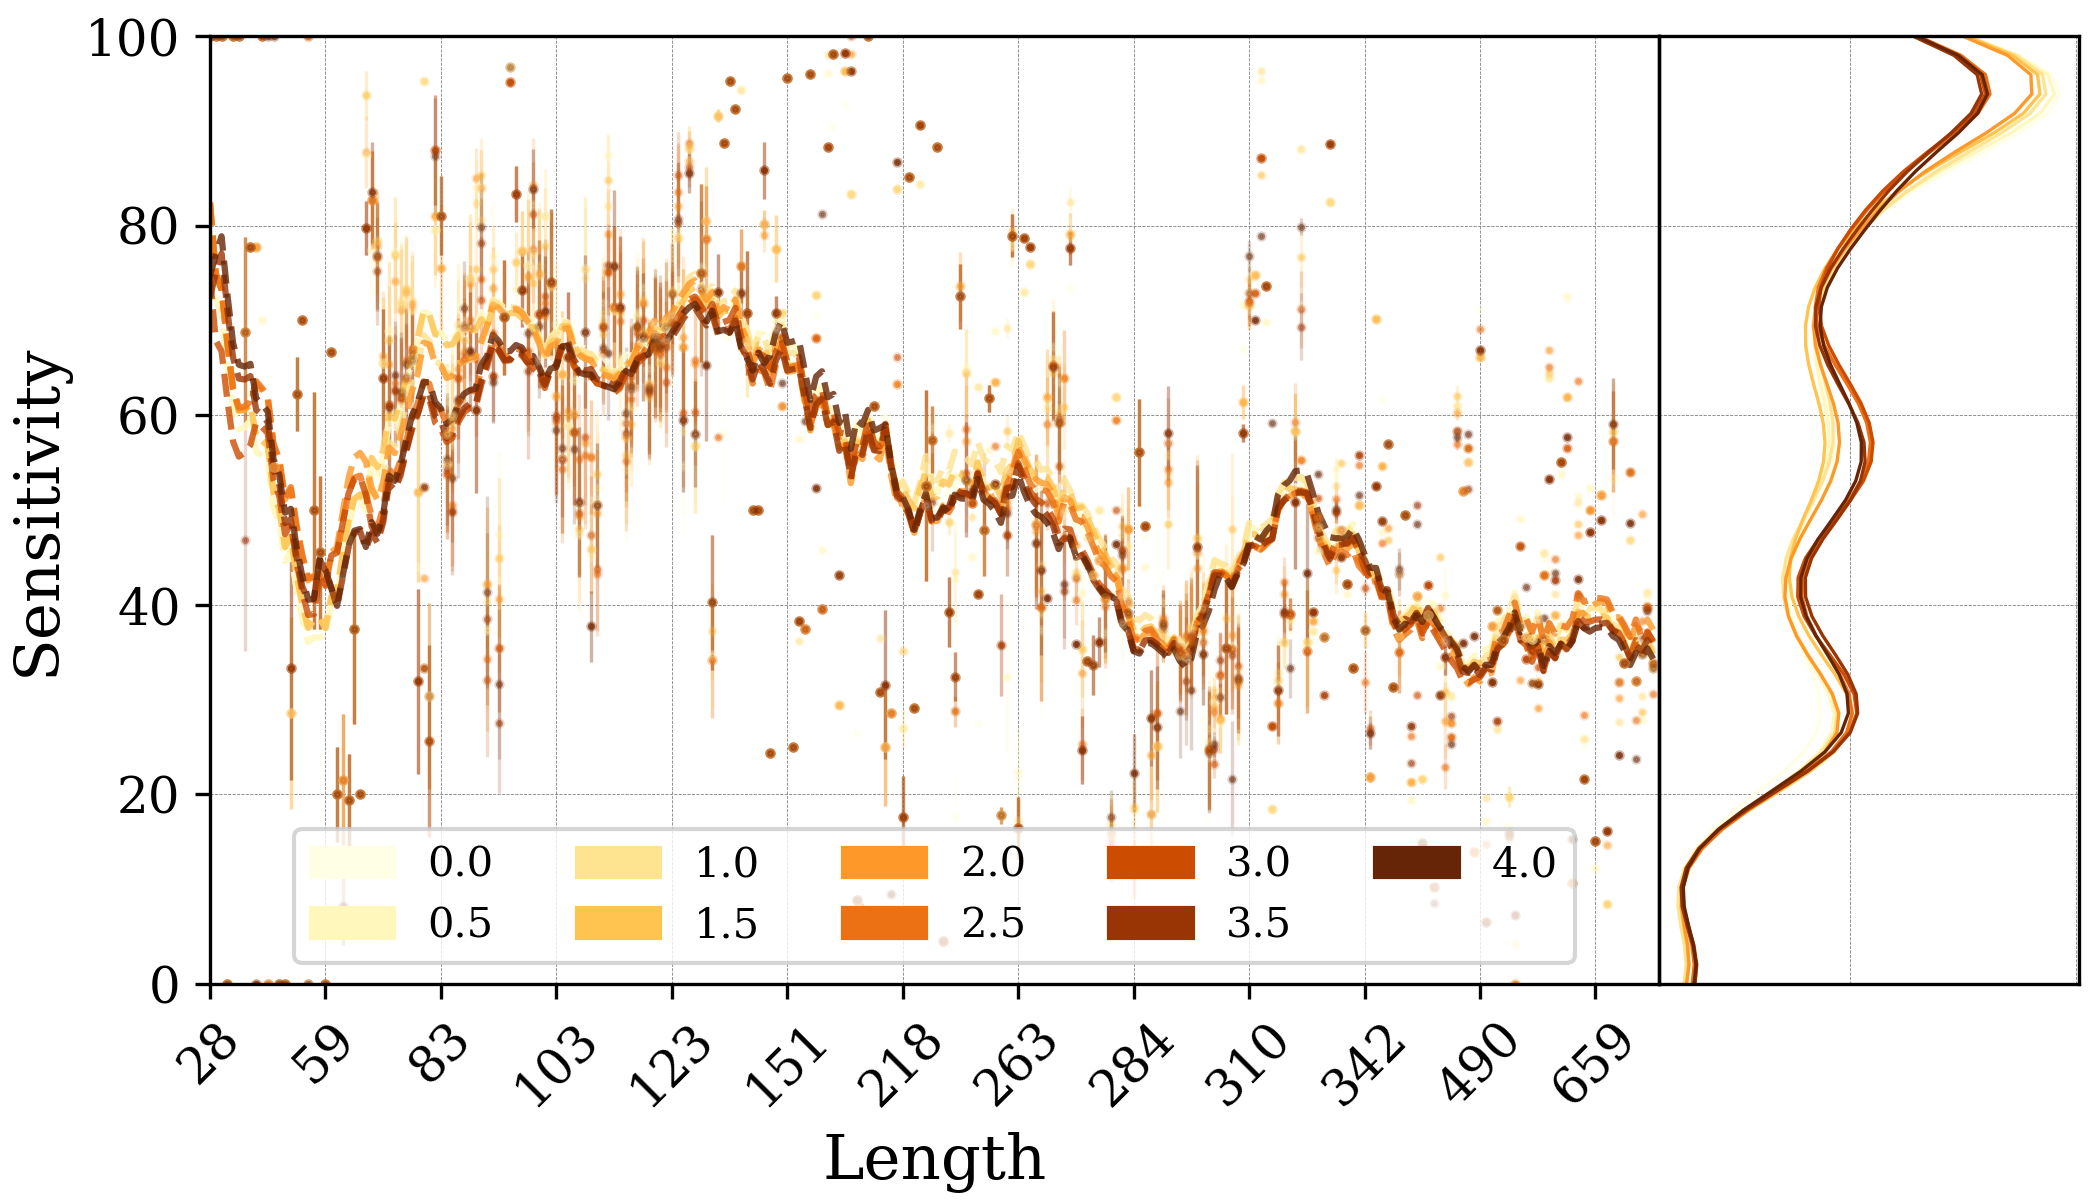
\includegraphics[scale=.7]{../res/images/rafft/rafft_perf_sens_minenergy.png}}
	\caption{\textbf{Predictive performance of RAFFT with various values of minimum energy contribution required for loop formation\label{app:perf_min_energy}.}
	Positive values for this parameter causes RAFFT to accept destabilizing loops, therefore being less greedy than per default. The performance of RAFFT was not observed to be positively affected by allowing sub-optimal loop formation.}
\end{figure}

\section{Percentage of correct base-pairs well predicted}
We analyse in this section the performance of \texttt{RAFFT} compared to both \ac{MFE} (\texttt{RNAfold}) and \ac{ML} (\texttt{Mxfold2}) predictions in terms of percentage of correct base-pairs predicted.
\begin{figure}[H]
	\centering
	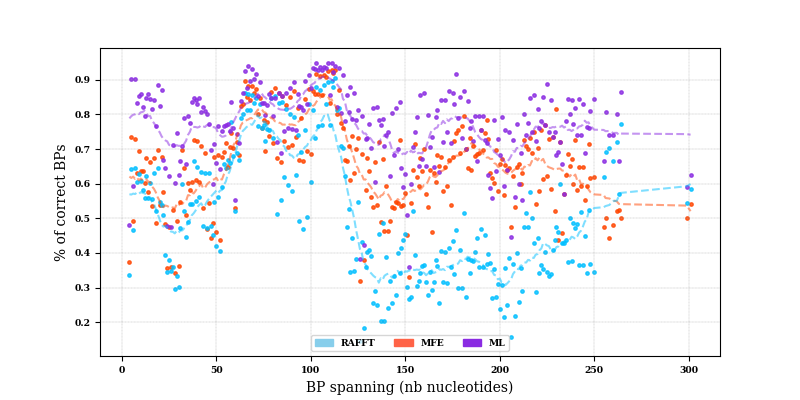
\includegraphics[width=1.\linewidth]{../res/images/rafft/bp_spanning.png}
	\caption{\textbf{Base pair spanning.} It shows the percent of base pairs predicted found in the known structures per number of nucleotides between them.}
\end{figure}

\section{Some Secondary structures with long unpaired regions}
To investigate the region of the structure space where the thermodynamic model tends to fail, we computed the composition of the known structures. Loop type lengths were computed in percentages. \autoref{perf_pca} shows those compositions' \ac{PCA}. From the \ac{PCA}, we observed that the known structures are distributed in the structure space toward interior loops. Also, some natural structures, as shown in figure \ref{diff_struct}, have large unpaired loops. The centre of mass in the principal component space is located in between the high-density stacking and interior loops. This shows that the dataset contains many elongated structures.
\begin{figure}[t!]
	\centering
	\subfloat[\texttt{srp\_Synt.wolf.\_CP000448}]{
		\begin{tikzpicture}
		\node (s11) at (0cm,3cm) {\subfloat[RAFFT]{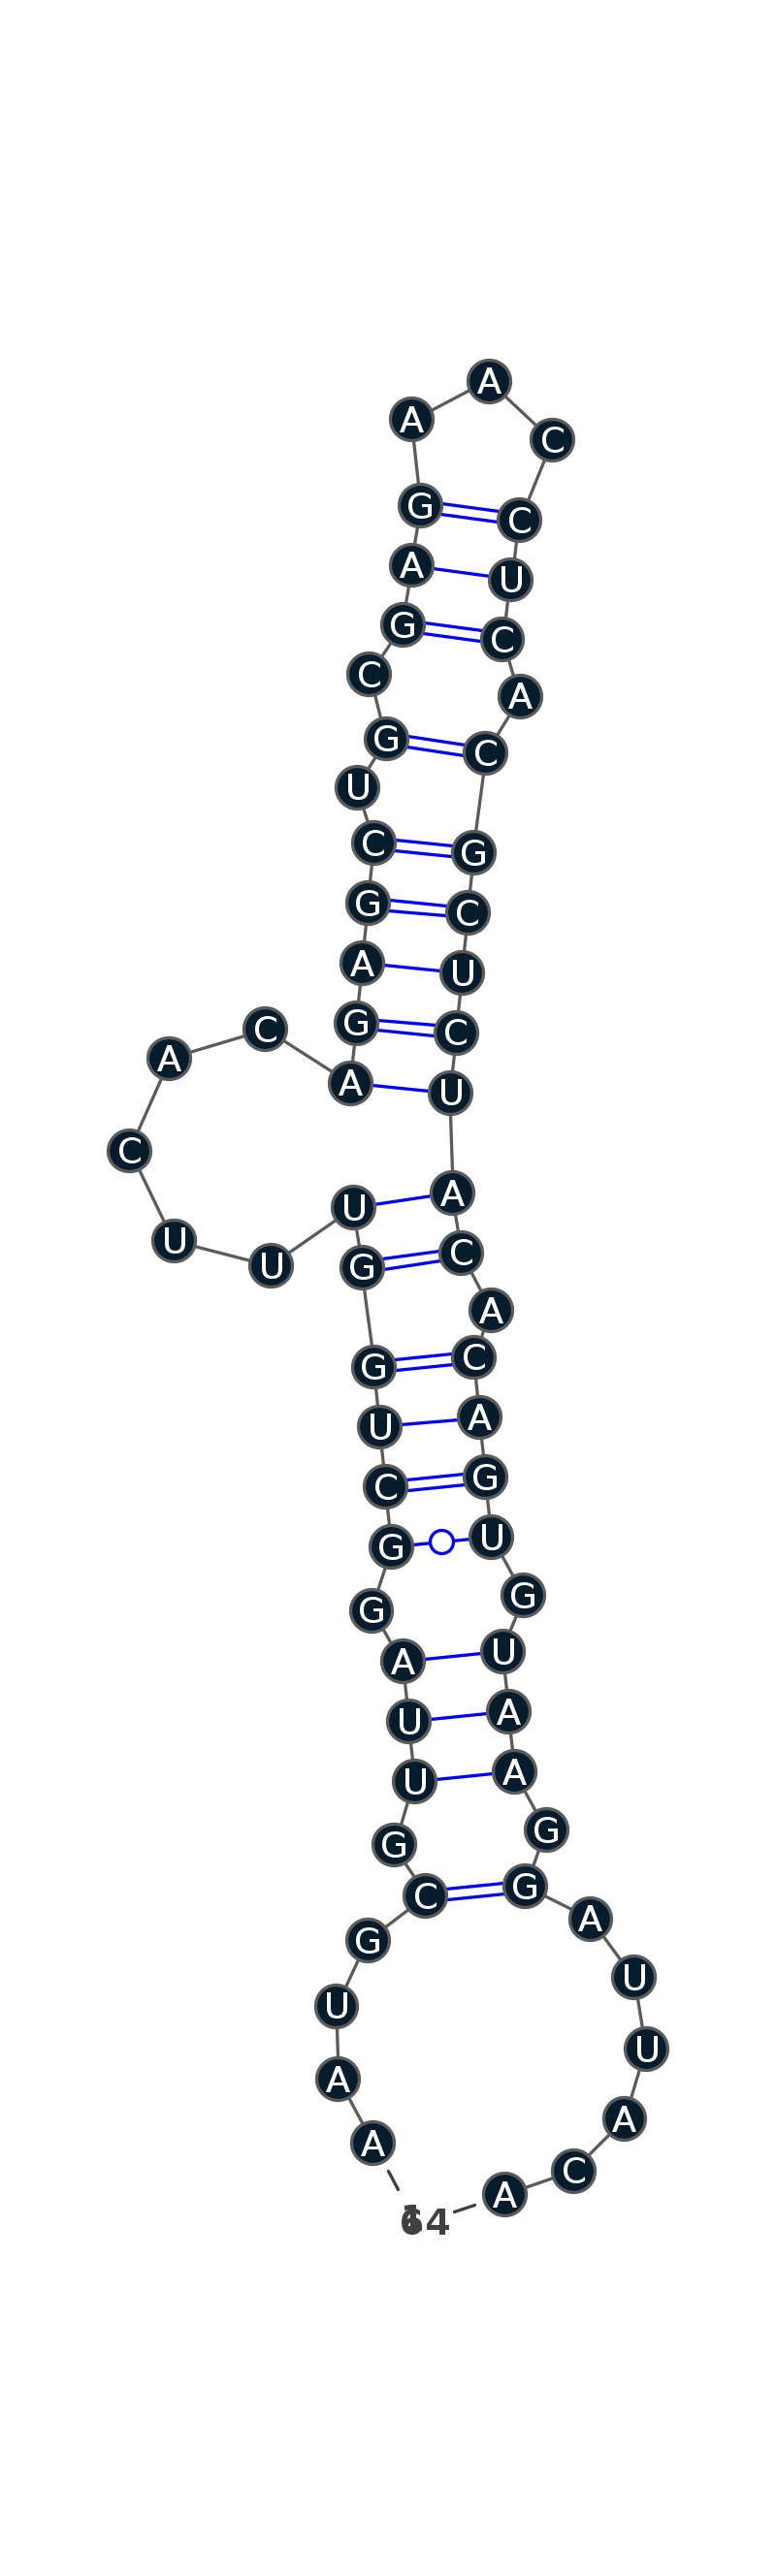
\includegraphics[scale=0.04]{../res/images/rafft/illed_img/srp_Heli_fft.png}}};
		\node (s12) at (3cm,3cm) {\subfloat[MFE]{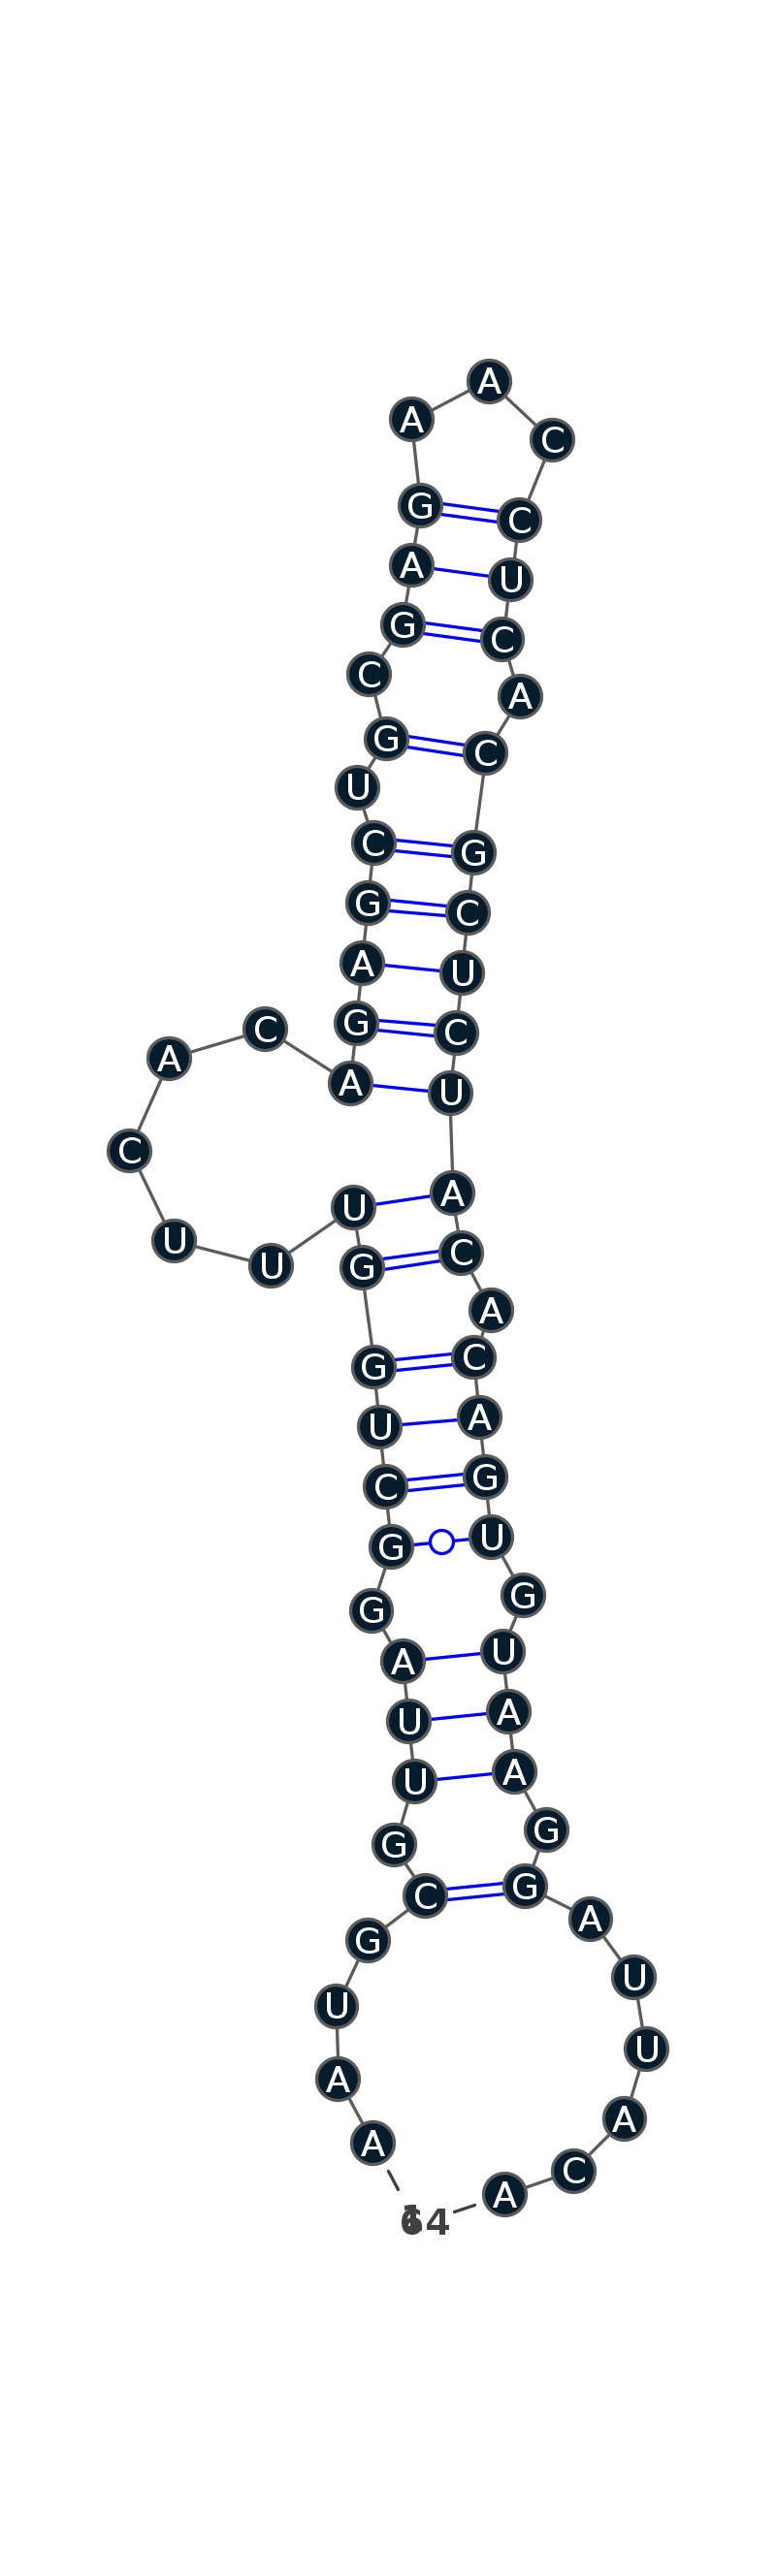
\includegraphics[scale=0.04]{../res/images/rafft/illed_img/srp_Heli_mfe.png}}};
		\node (s13) at (0cm,0cm) {\subfloat[ML]{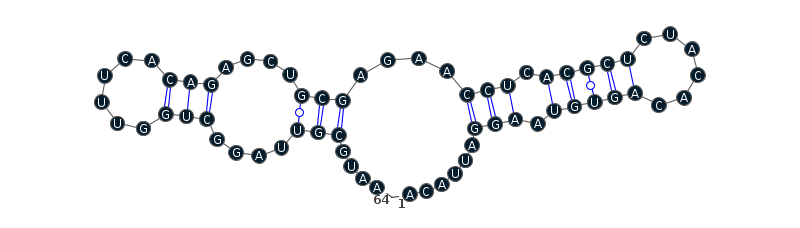
\includegraphics[scale=0.09]{../res/images/rafft/illed_img/srp_Heli_mle.png}}};
		\node (s14) at (3cm,0cm) {\subfloat[Native]{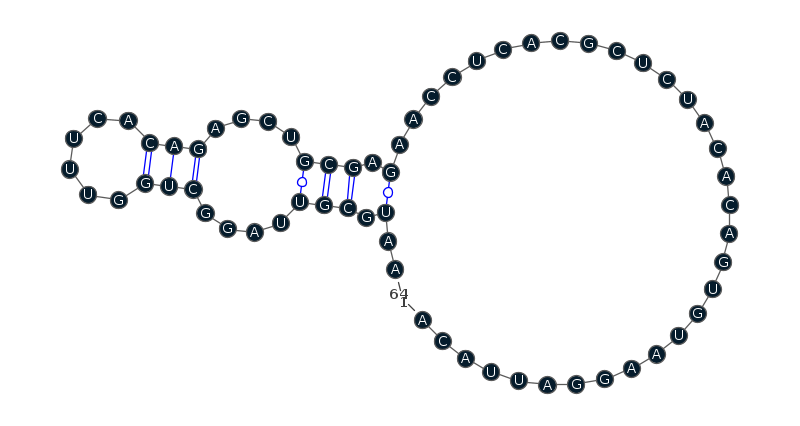
\includegraphics[scale=0.09]{../res/images/rafft/illed_img/srp_Heli_wts.png}}};
		\end{tikzpicture}
	}
	\subfloat[\texttt{srp\_Meth.mari.\_CP000745}]{
		\begin{tikzpicture}
		\node (s11) at (0cm,3cm) {\subfloat[RAFFT]{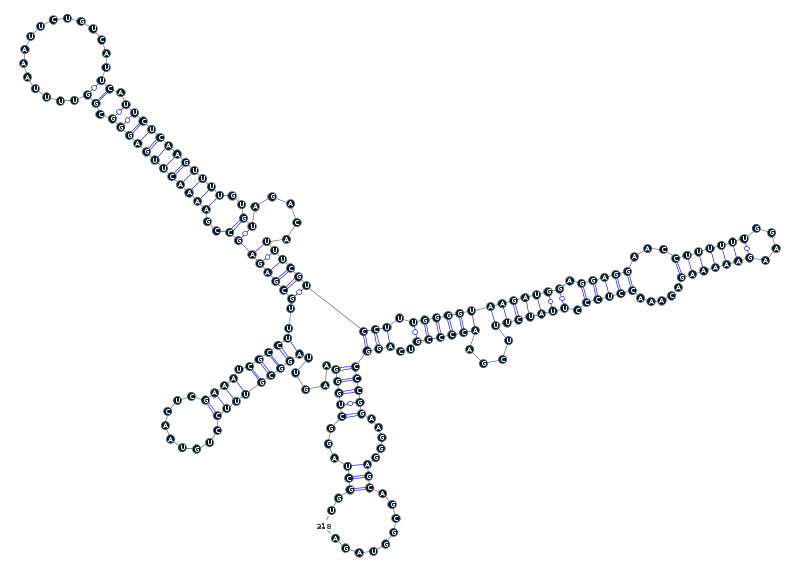
\includegraphics[scale=0.10]{../res/images/rafft/illed_img/srp_Meth_fft.png}}};
		\node (s12) at (3cm,3cm) {\subfloat[MFE]{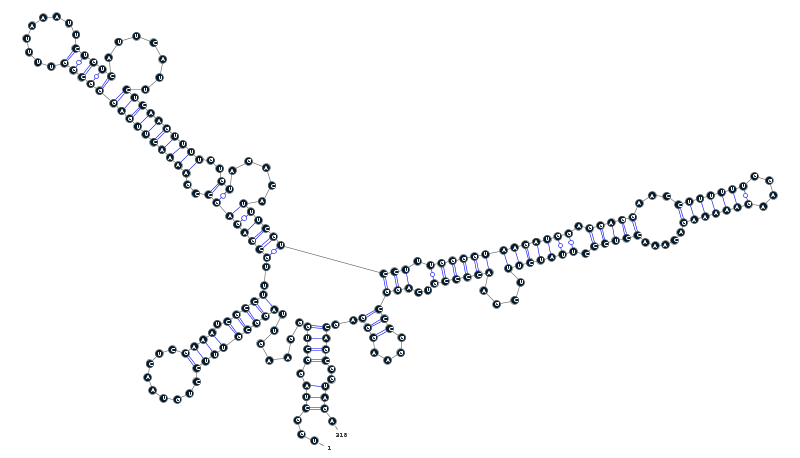
\includegraphics[scale=0.10]{../res/images/rafft/illed_img/srp_Meth_mfe.png}}};
		\node (s13) at (0cm,0cm) {\subfloat[ML]{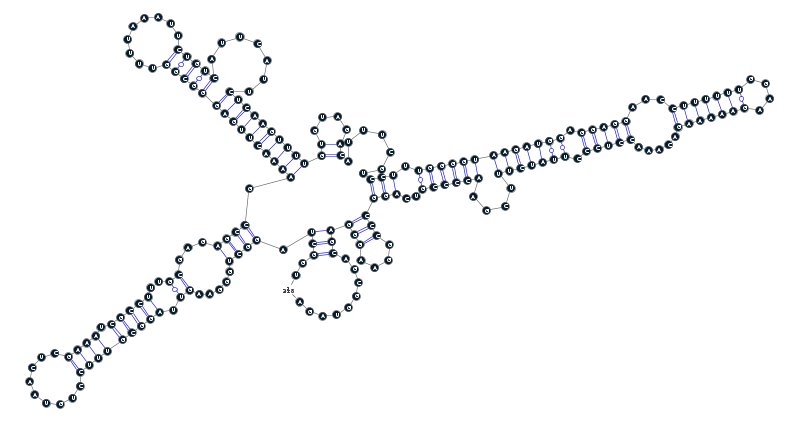
\includegraphics[scale=0.10]{../res/images/rafft/illed_img/srp_Meth_mle.png}}};
		\node (s14) at (3cm,0cm) {\subfloat[Native]{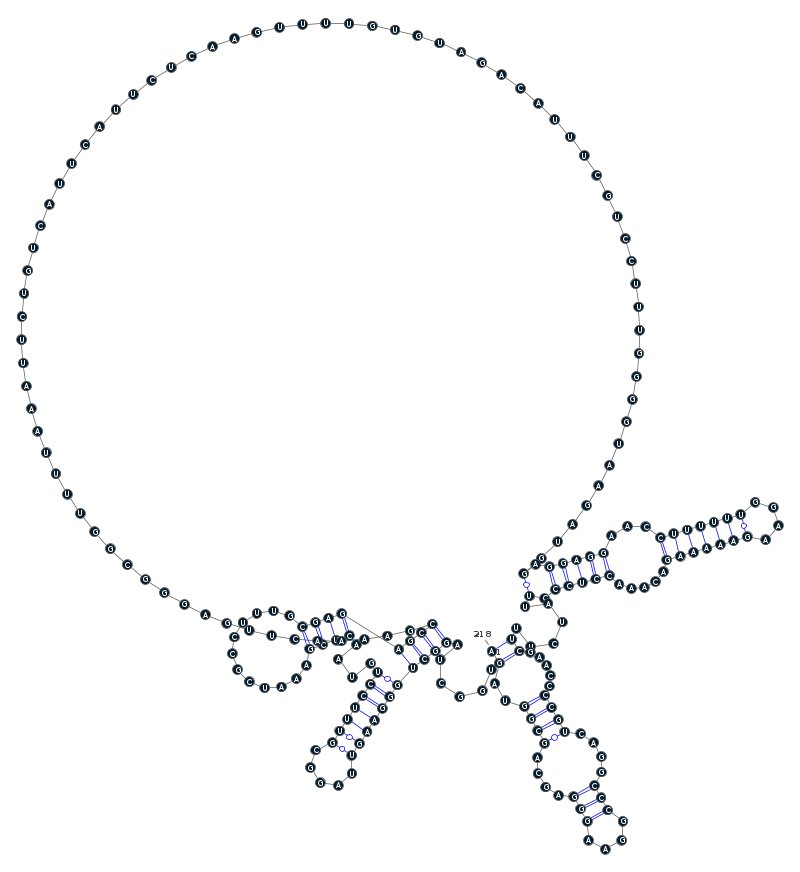
\includegraphics[scale=0.10]{../res/images/rafft/illed_img/srp_Meth_wts.png}}};
		\end{tikzpicture}
	}\\
	\subfloat[\texttt{tmRNA\_Cyan.mero.\_AY286123\_1\-236}]{
		\begin{tikzpicture}
		\node (s11) at (0cm,0cm) {\subfloat[RAFFT]{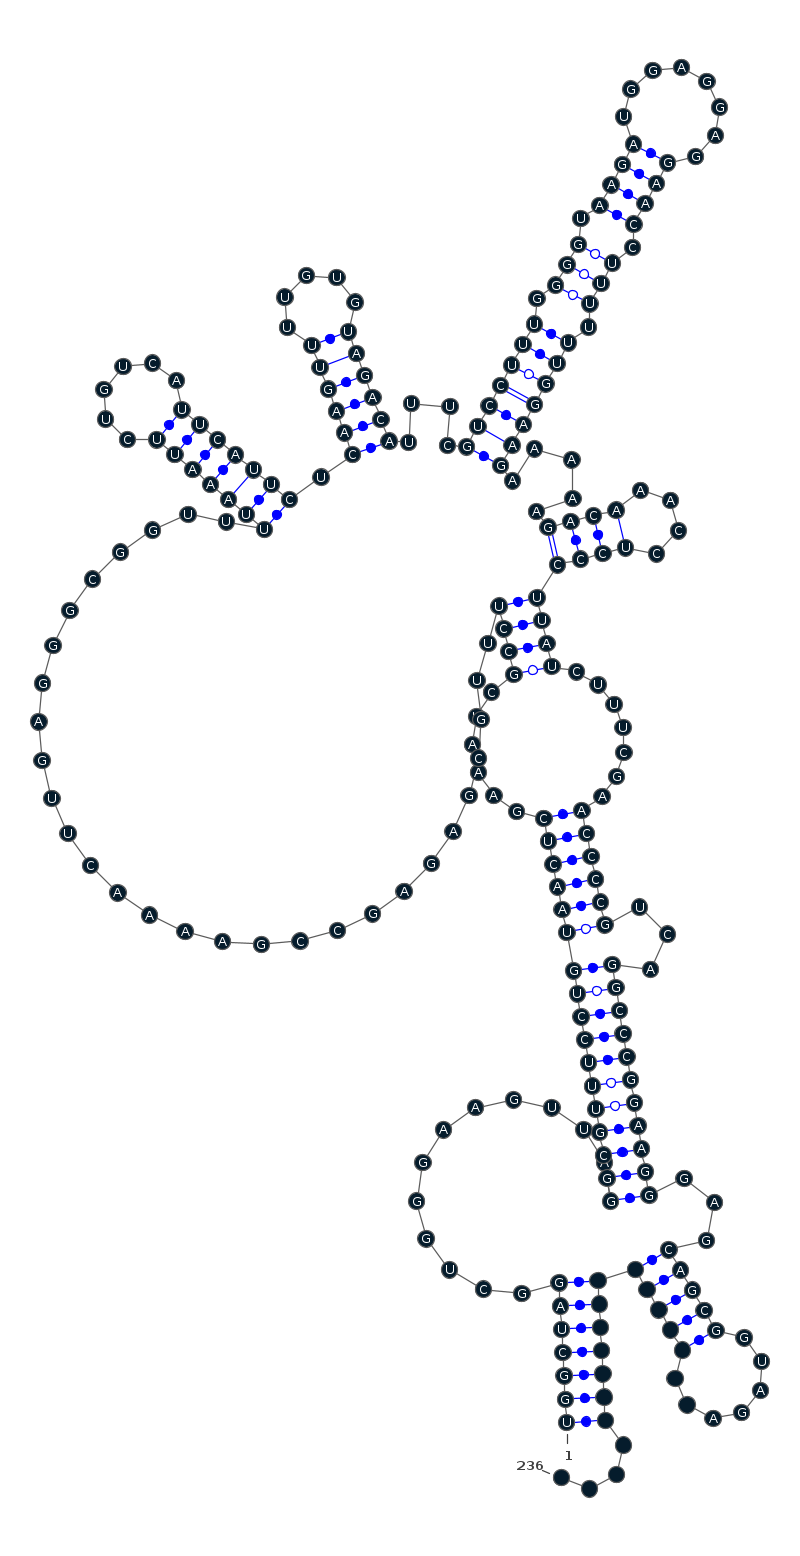
\includegraphics[scale=0.08]{../res/images/rafft/illed_img/tmRNA_Cyan_fft.png}}};
		\node (s12) at (3cm,0cm) {\subfloat[MFE]{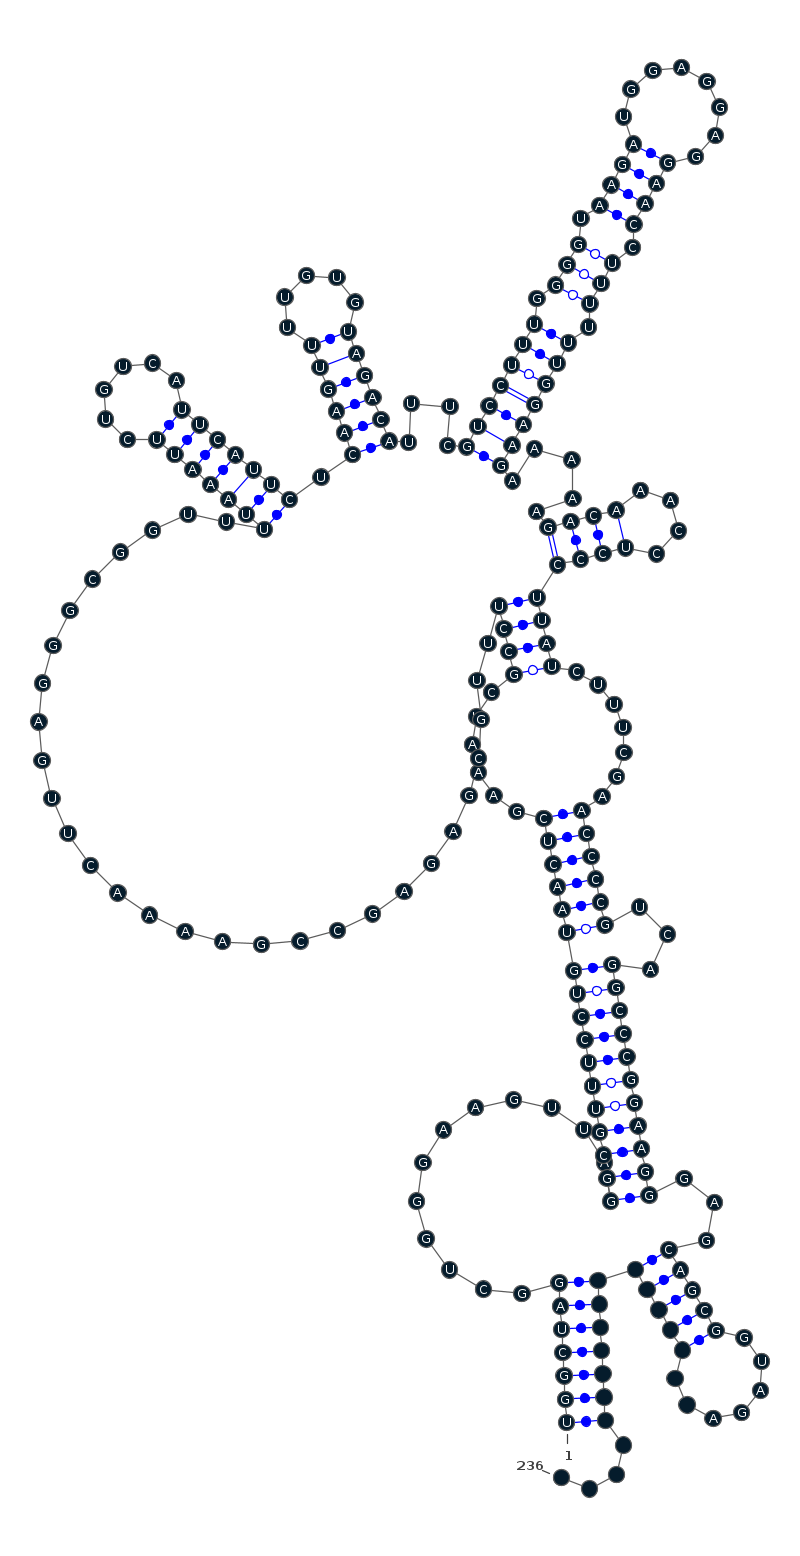
\includegraphics[scale=0.08]{../res/images/rafft/illed_img/tmRNA_Cyan_mfe.png}}};
		\node (s13) at (6cm,0cm) {\subfloat[ML]{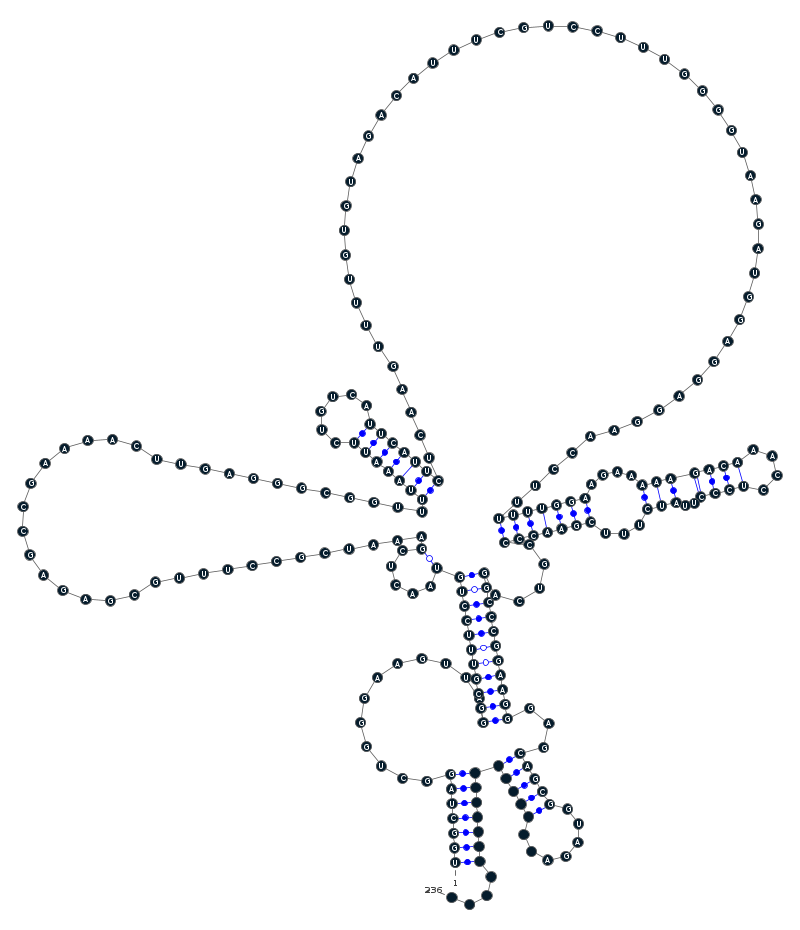
\includegraphics[scale=0.1]{../res/images/rafft/illed_img/tmRNA_Cyan_mle.png}}};
		\node (s14) at (9cm,0cm) {\subfloat[Native]{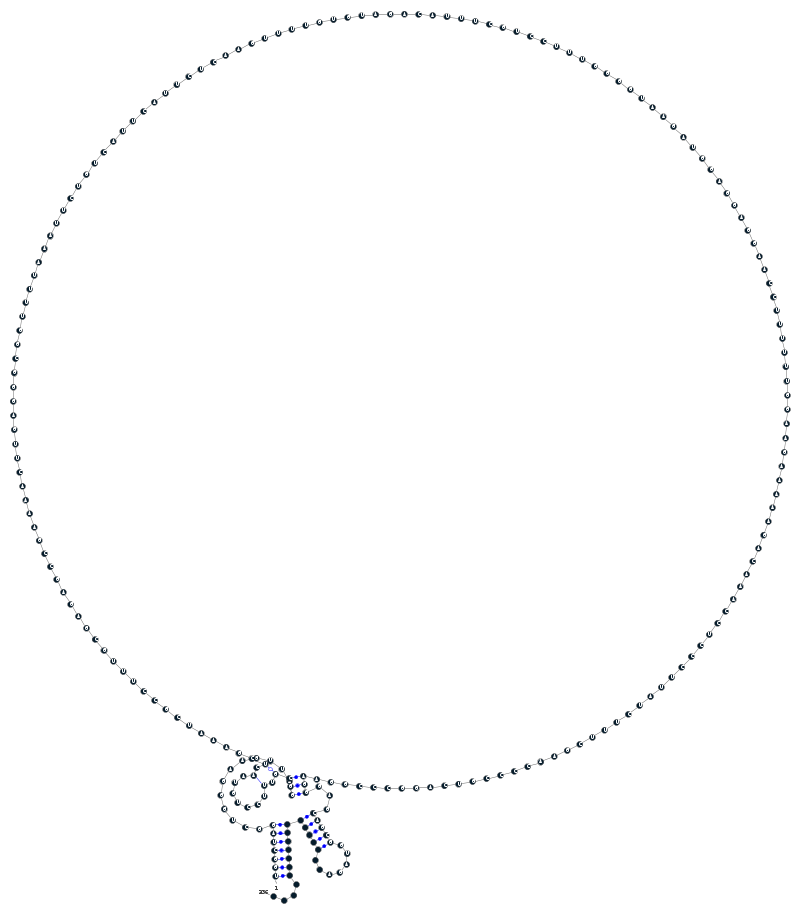
\includegraphics[scale=0.1]{../res/images/rafft/illed_img/tmRNA_Cyan_wts.png}}};
		\end{tikzpicture}
	}
	
	\caption{\textbf{Structures found to be difficult to predict with the thermodynamic model.} The sequence name where extracted directly from the dataset. Native is the known structure.\label{diff_struct}}
\end{figure}

